\documentclass{beamer}[10]


%
% macro
%

\usepackage{pgf}
\usepackage[english]{babel}
\usepackage[utf8]{inputenc} % use unicode chars
\usepackage{lmodern}% http://ctan.org/pkg/lm
\usepackage{beamerthemesplit}
\usepackage{graphics,epsfig,subfigure}
\usepackage{url}
\usepackage{srcltx}
\usepackage{hyperref}
\usepackage[mathescape,escapeinside=||]{minted}
\usepackage{import}
\usepackage{mathtools}
\usepackage{amsmath}
\usepackage{color}
%\usepackage[beamer]{hf-tikz}
\usepackage{xfrac}
\usepackage{makeidx}
\usepackage{multicol}

%\showboxdepth=5
%\showboxbreadth=5

% Slides in 16:9
\usepackage[orientation=landscape,size=custom,width=16,height=9,scale=0.5,debug]{beamerposter} 

%
% Macros
%
\definecolor{darkred}{rgb}{0.55, 0.0, 0.0}
\definecolor{light-gray}{gray}{.80}
\definecolor{light-yellow}{rgb}{255,255,153}
\definecolor{alizarin}{rgb}{0.82, 0.1, 0.26}
% colorized font
\newcommand{\red}[1] {{\color{red} #1}}
\newcommand{\darkred}[1] {{\color{darkred} #1}}
\newcommand{\blue}[1] {{\color{blue} #1}}
\newcommand{\green}[1] {{\color{green} #1}}
\newcommand{\gray}[1] {{\color{gray} #1}}
\newcommand{\grey}[1] {{\color{gray} #1}}

\newcommand{\hearts} {\red{$\heartsuit$}}
\newcommand{\diamonds} {\red{$\diamondsuit$}}
\newcommand{\spades} {$\spadesuit$}
\newcommand{\clubs} {$\clubsuit$}
\newcommand{\pyoptional}[1]{\diamonds #1 \diamonds}

\newcommand{\deltasum}[1]{\sum (#1 - \bar{#1})}
\newcommand{\deltasumsq}[1]{\sum (#1 - \bar{#1})^{2}}

%
% Take care of the newline after \frametitle
%
\newenvironment{pyframe}[1]
{\begin{frame}[fragile,environment=pyframe]\frametitle{#1}
 
}
{\end{frame}}


% environments
\newminted{py}{mathescape,escapeinside=||}% 
\newminted{bash}{mathescape,escapeinside=||}%

% python highlights: module, method
\newcommand{\pymodule}[1]{\darkred{\textbf{#1}}}
\newcommand{\pyfunction}[1]{\textit{#1}}
\newcommand{\keyword}[1]{\texttt{#1}}
\newcommand{\pyver}[1]{\colorbox{yellow}{#1}}
\newcommand{\typeonly}[1]{\colorbox{green}{#1}}
\newcommand{\pyvers}[1]{\raisebox{0em}{\colorbox{yellow}{#1}}}
\newcommand{\code}[1] { \texttt{#1} }

% special symbils
\newcommand{\mymapsto}{\operatornamewithlimits{\longmapsto}}

\makeatletter
\newcommand{\xMapsto}[2][]{\ext@arrow 0599{\Mapstofill@}{#1}{#2}}
\def\Mapstofill@{\arrowfill@{\Mapstochar\Relbar}\Relbar\Rightarrow}
\makeatother




%
% style
%

\setbeamercovered{transparent}
\mode<presentation>

%\geometry{top=5pt, margin=5pt}
%The outertheme defines the head and the footline of each slide
% \setbeamercolor{block title}{bg=orange}
% \useinnertheme{circles}
% \useoutertheme{split}
%\beamertemplatenavigationsymbolsempty

%\usetheme[numbers,totalnumber,compress,sidebarshades]{Babel}
\setbeamertemplate{headline}{
 \leavevmode%
  \hbox{%
%,bb=0 0 5cm 2cm
    \hspace{5pt}\includegraphics[height=1.2cm]{logo.eps}
    \hspace{240pt}\includegraphics[height=1.2cm]{logo.eps}
    }
}
\setbeamertemplate{footline}{
\noindent\textbf{\hspace{5pt}\insertsection \insertsubsection\hfill}\textbf{\hfill{\color{gray}\insertshortauthor}\hfill}\textbf{\hfill }
   % \textline[t]{ \insertsection  \insertsubsection}{\gray{\insertshortauthor}}{right}
}
%\useinnertheme[shadow=false]{rounded}
% frametitle
\setbeamertemplate{frametitle}[default][center]
\setbeamercolor*{frametitle}{bg=white,fg=gray,parent=palette primary}
\setbeamerfont{frametitle}{series=\bfseries,size={\fontsize{16}{8}}}
% table of contents
\setbeamercolor{section in toc}{fg=black} % series=\bfseries,size={\fontsize{16}{8}}}
%\setbeamercolor{section/subsection in toc}{fg=black}
%\setbeamercolor{subsection in toc}{fg=black}
%\setbeamerfont{section in toc}{fg=black} % series=\bfseries,size={\fontsize{16}{8}}}
%\setbeamerfont{section/subsection in toc}{fg=black}
%\setbeamerfont{subsection in toc}{fg=black}

%title
\setbeamercolor{title}{fg=black,bg=white}
\setbeamerfont{title}{series=\bfseries,size={\fontsize{24.88}{32}}}
%subtitle
\setbeamercolor{subtitle}{fg=gray}
\setbeamerfont{subtitle}{series=\bfseries,size={\fontsize{14}{}}}
%titlepage
\setbeamertemplate{title page}[default][center]
% bullets
\setbeamercolor{itemize item}{fg=gray}
\setbeamertemplate{itemize items}[circle]
\setbeamercolor{itemize item}{fg=light-gray}
\setbeamercolor{itemize items}{fg=light-gray}
% enumerations
\setbeamercolor{enumerate item}{fg=black}
\setbeamercolor{local structure}{fg=black}

%
% increase itemize spacing
%
%\newlength{\wideitemsep}
%\setlength{\wideitemsep}{\itemsep}
%\addtolength{\wideitemsep}{14pt}
%\let\olditem\item
%\renewcommand{\item}{\setlength{\itemsep}{\wideitemsep}\olditem}

  % \usecolortheme[named=orange]{structure}
  % \useinnertheme{circles}
  % \usefonttheme[onlymath]{serif}
\setbeamercovered{transparent}
  % \setbeamertemplate{blocks}[rounded][shadow=true]

\makeindex


% Apply DRAFT watermark
\usepackage{draftwatermark}
\setbeamercolor{background canvas}{bg=}%transparent canvas

\title{Orchestrating MySQL with Python and Docker}
\subtitle{EuroPython 2015, $22^{th}$ July - Bilbao}
\author{Roberto Polli - \href{mailto:roberto.polli@par-tec.it}{roberto.polli@par-tec.it}}
\date{21-27 July 2015}
\institute{Par-Tec Spa - Rome Operation Unit\\
    P.zza S. Benedetto da Norcia, 33\\
    00040, Pomezia (RM) - www.par-tec.it}

%
%
\begin{document}

%% cover
\frame{\titlepage 
\vspace{-0.5cm}
}


%% agenda
\iffalse
\frame{\frametitle{Agenda}
\tiny
\tableofcontents%[pausesection]
}
\fi

%% Starting doc
\section{Intro}
\frame{ \frametitle{Who? What? Why?}
\begin{itemize}

\item Manage, replicate, scale and provision MySQL databases with python fabric
\\
\\
\item Roberto Polli - Solutions Architect @ par-tec.it. Loves writing in C,
Java and Python. Red Hat Certified Engineer and Virtualization
Administrator.
\\
\\
\item Par-Tec – Proud sponsor of this talk ;) Contributes to various FLOSS. \\
Provides expertise in IT Infrastructure \& Services and \\ Business Intelligence
solutions + Vertical Applications for the financial market.

\end{itemize}
}

\begin{pyframe}{Agenda}
\begin{itemize}
\item Setup environment
\item Docker \& Compose
\item MySQL 5.6+ Replication
\item Fabric overview
\item Installing fabric
\item High Avalability \& Failover
\item Creating a Docker Provisioning driver
%\item modules: \pymodule{scipy, matplotlib}
\end{itemize}
\end{pyframe}

%
%
%
\begin{pyframe}{Setup}
Install Docker
\begin{bashcode}
sudo apt-get install lxc-docker || \
yum -y install docker
\end{bashcode}
Download the course scripts
\begin{bashcode}
git clone https://github.com/ioggstream/mysql-community
cd mysql-community/fabric
\end{bashcode}
Install requirements and setup environment
\begin{bashcode}
pip install -r requirements.txt
docker-compose up
\end{bashcode}
\end{pyframe}


%
% Docker 101
%
\section{Docker}
\begin{pyframe}{Docker}
A brief docker tutorial based
on the busybox image.
Setting images, hostnames and environment variables.
\begin{bashcode}
$ docker run [--rm] -ti --name=test busybox /bin/bash
$ docker exec -ti  test /bin/bash
...
\end{bashcode}
OT: nat, entrypoint, ...
\end{pyframe}

\section{Docker}
\begin{pyframe}{Docker Compose}
A brief docker-compose tutorial:
describing containers via yml
\\
Running the provided services
using docker-compose.
\\
Scaling services with compose.
\\
If audience is confident with compose, a patch
for customizing hostnames of docker-compose scale is presented.

\end{pyframe}

%
% MySQL
%
\section{MySQL}
\begin{pyframe}{MySQL Replication 101}
Advantage of replication:
\begin{itemize}
  \item  scaling reads
  \item  high availability
  \item ease of backup
\end{pyframe}


\begin{pyframe}{MySQL Replication 101}
Overview of MySQL Replication:
\begin{itemize}
\item master creates a changelog (binlog),
% by default binlog never expires
\item slaves download and apply it.
\item Global Transaction ID.
\item Asynchronous and Semi-Synchronous replication.
\end{itemize}
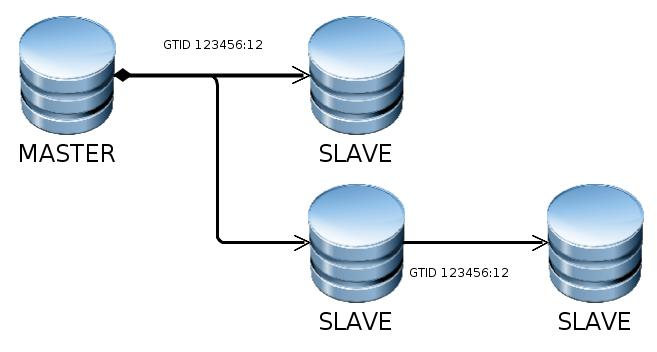
\includegraphics[height=4cm]{images/mysql-propagate-gtid.jpg}
\end{pyframe}


\iffalse
\begin{pyframe}{Replication 2.0}
MySQL 5.6+ replication is based on Global Transaction ID
\begin{itemize}
\item Every server has a unique UUID \\
\code{3E11FA47-71CA-11E1-9E33-C80AA9429562}

\item This makes every TransactionID a Global one
\code{3E11FA47-71CA-11E1-9E33-C80AA9429562:32}
\end{itemize}
GTIDs avoid loops in replication!
\end{pyframe}


\begin{pyframe}{Configuring replication}
\begin{itemize}
\item In MySQL replication is configured on the slave only.
\item The slave connects to the master with a provisioned
 user and gets its changelog (binlog).
\end{itemize}
%% IMAGE
If binlog had been purged, you need to import the
master database first!
\end{pyframe}
\fi


\begin{pyframe}{MySQL Replication 101}
Running mysql with the provided my-gtid.cnf.
Replication arguments: server-id, binlog, relaylog, ...
Create a master-slave replication agreement.
\code{SLAVE START; SLAVE STOP; SHOW SLAVE STATUS \G; SHOW MASTER STATUS;}
\end{pyframe}


\begin{pyframe}{MySQL Replication 101}
mysqlreplicate takes care of
\begin{itemize}
\item provisioning the replica user on the master;
\item configure the slave to point to the master.
\end{itemize}
\begin{minted}
mysqlreplicate \
 --master=root:pass@master \
 --slave=root:pass@slave \
 --rpl-user=repl:rpass \
 -b

# master on 192.168.1.1: ... connected.
# slave on 192.168.1.2: ... connected.
# Checking for binary logging on master...
# Setting up replication...
# ...done.
\end{minted}
\end{pyframe}


%
% Fabric
%
\begin{pyframe}{Fabric - HLA}
Fabric is a python framework for managing, replicating, sharding and scaling mysql clusters.
\begin{itemize}
\item tie servers in high availability groups
\item configure single-master replication topologies
\item monitor failures
\item proxy for rw/split and sharding
\end{itemize}
\end{pyframe}
%http://mysqlmusings.blogspot.it/2013/10/mysql-fabric-high-availability-groups.html


\begin{pyframe}{Fabric - HLA}
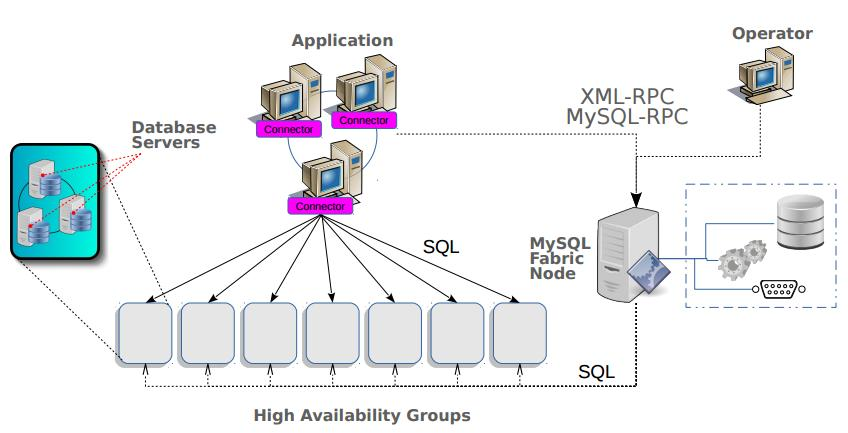
\includegraphics[height=6.6cm,width=12cm]{images/mysql-fabric-hla.jpg}
\end{pyframe}


\begin{pyframe}{Fabric \& Python Utilities - get it}
Python 2.7
    \begin{bashcode*}
    wget |\href{https://dev.mysql.com/get/Downloads/MySQLGUITools/mysql-utilities-1.6.1.tar.gz}{http://bit.ly/1CxNuZe}|
    tar xf mysql-utilities-1.6.1.tar.gz
    python setup.py install
    \end{bashcode*}
Fedora / CentOS / RHEL 7
    \begin{bashcode}
    yum -y install \href{https://dev.mysql.com/get/mysql-community-release-el7-5.noarch.rpm}{http://bit.ly/1yhSViu} # MySQL Community repo
    yum -y install mysql-utilites
    \end{bashcode}
\end{pyframe}


\subsection{Setup - I}
Setup Fabric Server.
We will access all servers from this container
which includes *all* mysql tools and utilities.
\begin{bashcode}
$ docker-compose up -d
$ docker exec -ti fabric_fabric_1 /bin/bash
fabric$
\end{bashcode}
\end{pyframe}

\begin{pyframe}{Setup - II}
All settings (eg my.cnf) to avoid typing credientals
and establish pain-free communication between nodes.
 \\ \\
Students won't waste time.
\end{pyframe}


\begin{pyframe}{Installation}
Setup fabric server via fabric.cfg . \\
Testing fabric installation (database existence, mysqlfabric ping, ..)

\begin{bashcode}
$ mysqlfabric ping ...
\end{bashcode}
\end{pyframe}


\section{High Availability Group}
\begin{pyframe}{High Availability Group}
Create a replication group and adding
servers. \\

Promoting one server as a master. \\

Monitoring failover. \\
\begin{bashcode}
# mysqlfabric group ...
\end{bashcode}
\end{pyframe}


\begin{pyframe}{Troubleshooting replication}
Using python mysql-utilities to provision
 a new slave when binlogs are not complete. \\

 Caveats on big databases. \\


\begin{bashcode}
# mysqldbexport / mysqldbimport
\end{bashcode}
\end{pyframe}


\iffalse
    \begin{pyframe}{Provisioning a new master}
    You can provision a new slave creating a suitable dump
    with mysqldbexport. Just:
    \begin{itemize}
    \item check that replica user is provisioned on the master;
    \item create a custom dump.sql;
    \item add --export=master;
    \end{itemize}
    \begin{minted}
    cat > data.sql <<EOF
    -- ignore previous changelogs
    -- and trust the backup only
    STOP SLAVE;
    RESET MASTER;
    COMMIT;

    EOF

    mysqldbexport >> data.sql \
     --server=root:pass@master \
     --rpl-user=repl:rpass \
     --export=master \
     --rpl=master \
     --all

    mysqldbimport --server=root:root@slave \
     data.sql
    \end{minted}
    \end{pyframe}
\fi


\section{Failover}
\begin{pyframe}{Enabling and Testing Failover}
Enabling failover and stopping a master. \\

Re-ingesting a failed master. \\

\begin{bashcode}
#
\end{bashcode}
\end{pyframe}


\section{Provisioning}
\begin{pyframe}{Provisioning new container via docker}
Show the provisioning interface (docker, openstack). \\

Provisining and deleting containers. \\

Adding provisioned container to ha groups. \\

\begin{pycode}
from mysql.fabric.providers import dockerprovider

# the MachineManager class...

\end{pycode}
\end{pyframe}




\iffalse
\begin{pyframe}{Title}
\begin{bashcode}
#
\end{bashcode}
\end{pyframe}
\fi




\begin{pyframe}{Wrap Up}
\begin{itemize}
\item Try Fabric with Docker!
\item Enjoy high availability!
\item Don't reingest failed master!
\end{itemize}
\end{pyframe}


\begin{pyframe}{That's all folks!}
\begin{center}
Thank you for the attention! \\\\
\insertauthor
\end{center}
\end{pyframe}


\end{document}
